\documentclass[11pt]{article}

\usepackage[T1]{fontenc}
\usepackage{lmodern}
\usepackage[a4paper,margin=2.5cm]{geometry}
\usepackage{amsmath,amssymb}
\usepackage{booktabs}
\usepackage{multirow}
\usepackage{graphicx}
\usepackage[expansion=false]{microtype}
% las referencias al articulo (M-...) se resuelven con su main.aux
\usepackage{xr-hyper}
\usepackage{hyperref}
\externaldocument[M-]{main}

\newcommand{\RE}{\mathrm{RE}}
\setlength{\emergencystretch}{3em}
\renewcommand{\thesection}{S\arabic{section}}
\renewcommand{\thetable}{S\arabic{table}}
\renewcommand{\thefigure}{S\arabic{figure}}
\renewcommand{\theequation}{S\arabic{equation}}

\begin{document}

\begin{center}
{\large\bfseries Supplementary material}\\[4pt]
Genetic Programming Hyper-Heuristics for the Job Shop Scheduling Problem
with Interval Durations: Robustness-Aware Interpretable Rules that
Generalize Across Instance Sizes
\end{center}

\noindent Sections, tables, figures and equations without the prefix S
refer to the article.

\section{Interval handling and the decoder}
\label{sec:decoder}

Two aspects of the comparison with the constructive baselines are
examined here: how each baseline reduces an interval to a comparable
quantity, and how much of the margin of the evolved rules belongs to
the priority rule rather than to the schedule generation scheme.

The baselines rank candidates by the lexicographic order of
Eq.~\eqref{M-eq:rank} (Section~\ref{M-sec:reference}). To check that this
choice does not handicap them, each interval-valued rule was re-run
ranking by a single number drawn from the same interval: its lower
endpoint, its midpoint or its upper endpoint. Over the 70 instances
SPT spans $633.1$ to $642.5$ across those three conventions, LPT
$703.1$ to $704.4$, MWKR $62.9$ to $64.6$ and EST $42.7$ to $45.1$. The
lexicographic values of Table~\ref{M-tab:baselines} are better than all
three for SPT and EST, and within $1.9$ points of the best for LPT and
MWKR. For EST and MWKR, the rules that account for the state of the
shop, no convention moves the result by more than $2.4$ points, and for
SPT and LPT, whose levels exceed 600, by at most $9.4$; the best plain
rule and the evolved one are $23.3$ points apart. How the intervals are
collapsed is therefore not what the comparison measures.

The decoder is a more substantial question, since the strongest
baseline, G\&T-MWKR, does not use the same one: it restricts each
decision to Giffler and Thompson's conflict set and so produces active
schedules, whereas the evolved rules choose from the whole eligible set
and produce semi-active ones. Running the evolved rules as the
tie-break \emph{inside} the conflict set separates the two effects.
Table~\ref{tab:decoder} gives the four combinations. Holding the
decoder fixed, the evolved rules outperform MWKR under either one: $18.99$
against $64.7$ in the semi-active decoder and $23.18$ against $29.5$
in G\&T's. Holding the rule fixed, each prefers a different decoder:
the evolved rules lose $4.2$ points when moved into the conflict set,
while MWKR gains $35.2$ by entering it. Each method in
Table~\ref{M-tab:baselines} is thus reported with the decoder that suits
it, and the margin survives the other choice.

\begin{table}[!htb]
\centering\small
\caption{RE (\%) over the 70 instances for the two decoders and the
two priority rules, one deterministic pass. The GP entries are the mean
over the 30 evolved rules.}
\label{tab:decoder}
\begin{tabular}{lcc}
\toprule
Priority rule & Semi-active & Giffler--Thompson \\
\midrule
MWKR & 64.7 & 29.5 \\
Evolved, mean of 30 & $\mathbf{18.99} \pm 1.33$ & $23.18 \pm 7.47$ \\
Evolved, featured & 17.71 & 18.15 \\
\bottomrule
\end{tabular}
\end{table}

Two details of the table deserve mention. The featured rule is
the one case where the decoder barely matters, $17.71$ against $18.15$,
a difference of $0.44$ points that a paired test over the 70 instances
does not separate from zero ($p = 0.32$); the loss is concentrated in
the rest of the arm, whose standard deviation grows from $1.33$ to
$7.47$ because a few rules deteriorate markedly once their candidate set is restricted. This is what should be expected of rules evolved against a
particular generation scheme: the conflict set removes candidates their
fitness was never measured on. And SPT, which is the worst entry of
Table~\ref{M-tab:baselines} at $627.2$, reaches $70.6$ inside the
conflict set, as G\&T-SPT, which is the same phenomenon seen from the
other side.

\section{Robustness under executional uncertainty: further analyses}
\label{sec:robdetail}

This section extends the robustness comparison of Section~\ref{M-sec:robustness} of the article, whose Table~\ref{M-tab:robustness} the paragraphs below refer to. It gives the paired tests behind that comparison and the per-instance distributions under widened intervals, removes the normalization of $\bar\varepsilon$, repeats the comparison at the level of the 30 rules of each arm, changes the law of the realizations, and describes the worst $5\%$ of executions.

The paired Wilcoxon tests behind the comparisons of the article, on $\bar\varepsilon$ at the nominal width, are the following.

Under the makespan objective the width terminals make no difference to
robustness either (Table~\ref{M-tab:robustness}): the featured rule and its
ablated counterpart are statistically indistinguishable in
$\bar\varepsilon$ ($5.70$ against $5.75$ at the nominal width; paired
Wilcoxon over the 70 instances, $z=-0.17$). The rule is more robust than
G\&T-MWKR ($6.29$, $z=-4.42$, $p<0.001$, $|r|=0.61$) but not than EST
($5.66$, $z=0.42$), although it improves on EST by $24.6$ points of
$\RE$; in absolute terms, which removes EST's larger expected makespan
from the denominator, the rule deviates by $12.30$ time units against
EST's $14.64$ ($z=-5.89$, $p<0.001$, $|r|=0.81$). A low deviation does
not require a low makespan, so robustness must be optimized for
directly.

The robust fitness achieves this. The narrowest rule of the
$\lambda{=}1$ arm reduces $\bar\varepsilon$ from $5.70$ to $4.52$
($z=-6.40$, $|r|=0.88$ against the makespan rule), and the reduction
requires the width terminals: under the same fitness, its ablated
counterpart reaches $5.54$ ($z=-6.25$, $|r|=0.86$). At $\lambda{=}4$ the
deviation falls to $4.21$. In absolute terms the reduction is $16.2\%$,
from $12.30$ to $10.31$ time units ($z=-5.55$, $p<0.001$, $|r|=0.76$),
so it does not come from the larger expected makespan in the
denominator. The narrower predicted intervals of
Section~\ref{M-sec:frontier} thus correspond to smaller realized
deviations, at the cost in expected makespan reported in the RE column:
$24.95$ and $28.27$ against $17.71$.

Methods can also be compared at similar levels of $\RE$, which
separates the robustness gain from the expected makespan given up for
it. The robust $\lambda{=}4$ rule and G\&T-MWKR predict almost the same
makespan, $2454$ against $2482$ time units, which is $28.27$ against
$29.50$ points of $\RE$. Their realized deviations differ markedly:
$9.78$ against $14.94$ time units, a reduction of $34.5\%$, smaller on
69 of the 70 instances ($z=-7.26$, $p<0.001$, $|r|=1.00$). At matched
a-priori quality the robustness gain is therefore neither a denominator
effect nor a makespan concession.

The comparison with EST reverses once the normalization is
removed. $\bar\varepsilon$ divides by $E[\mathbf{C}_{\max}]$, and EST's predicted
makespan is $21\%$ larger than the rule's ($2732$ against $2259$ time
units on average), so the same absolute error reads as a smaller
relative one. In absolute terms the rule deviates by $12.30$ time units
against EST's $14.64$, and the difference is significant ($z=-5.89$,
$p<0.001$, $|r|=0.81$). The ordering against G\&T-MWKR is unchanged and
widens ($12.30$ against $14.94$, $z=-6.83$, $|r|=0.94$), and the
makespan arm and its ablation remain indistinguishable ($12.30$ against
$12.25$, $z=0.61$, $p=0.55$). The normalization therefore conceals an advantage of the rule rather than creating one.

The reduction of $\bar\varepsilon$ that the robust fitness achieves in the article, from $5.70$ to $4.52$ for the narrowest rule of the $\lambda{=}1$ arm, is partly due to the denominator, and the absolute deviation quantifies it. The robust $\lambda{=}1$ arm carries an
$E[\mathbf{C}_{\max}]$ that is $6.1\%$ larger than the makespan arm's, so where
$\bar\varepsilon$ falls by $20.7\%$ the absolute deviation falls by
$16.2\%$, from $12.30$ to $10.31$ time units; at $\lambda{=}4$ it
reaches $9.78$. Roughly a fifth of the apparent gain is therefore
arithmetic and the rest is not: the paired contrasts are also significant on the absolute measure, by $-1.99$ time units against the makespan
arm ($z=-5.55$, $p<0.001$, $|r|=0.76$) and by $-1.78$ against its own
ablation ($z=-5.17$, $|r|=0.71$).

The comparisons above select one representative rule per arm; at the
level of the method the ordering is the same. Recomputing
$\bar\varepsilon$ at the nominal width for all 30 rules of each arm
and comparing the arms as independent samples, the makespan arm averages
$5.67 \pm 0.16$ against $5.77 \pm 0.14$ for its ablation
($z=-2.40$, $p<0.05$ after Holm's correction over the three
arm-level tests, $|r|=0.36$), the robust $\lambda{=}1$ arm
$5.50 \pm 0.30$ against $5.68 \pm 0.11$ for its own ($z=-2.91$,
$p<0.05$, $|r|=0.44$), and the robust arm improves on the
makespan arm with the same terminals ($z=-2.68$, $p<0.05$,
$|r|=0.40$).

Two things follow. The width terminals do reduce
$\bar\varepsilon$ slightly even under the makespan objective, a method-level effect too small to be detected in the single featured pair; and
the arm-level reductions are modest, three percent or less, against the
fifth separating the featured rules, so selecting the narrowest rule of
the robust arm amplifies an effect that at the method level is
consistent but small.

The estimate of the article draws each realization uniformly on its
interval, which is one choice among several. Repeating the measurement
with a symmetric triangular law, with a law skewed towards the upper
endpoint, and with the single worst-case realization in which every
duration takes its upper bound, leaves the ordering and every
significant contrast intact. Averaged over the 70 instances, the robust
$\lambda{=}1$ arm improves on the makespan arm by $1.22$ time units
under the triangular law, $12.16$ under the skewed one and $29.01$ in
the worst case, all with $p<0.001$; the makespan arm and its ablation
remain indistinguishable under all three. The deviations themselves
grow with the mass the law places near the upper endpoint, from $8.95$
time units for the rule under the triangular law to $57.15$ under the
skewed one and $138.35$ in the worst case, but the comparison between
methods does not depend on which law is used.

The measures above are averages over realizations, whereas a planner
exposed to late completions is concerned with the worst ones. The
conditional value-at-risk of Section~\ref{M-sec:stats}, computed on the
same $K{=}1000$ realizations, describes the $5\%$ worst executions of
each schedule and separates two questions. The first is how far those
executions exceed the prediction. Under the uniform law the featured
rule overruns its expected makespan by $33.46$ time units on average
over its worst $5\%$ of executions, against $38.87$ for G\&T-MWKR and
$40.81$ for EST ($z=-5.04$ and $z=-5.61$, $p<0.001$), and its ablated
counterpart is indistinguishable ($33.55$, $z=-0.05$). The robust
objective reduces the tail overrun in about the same proportion as the
mean deviation: to $27.46$ at $\lambda{=}1$, $17.9\%$ less than the
makespan rule ($z=-5.14$, $p<0.001$, $|r|=0.71$) and $5.68$ less than
its own ablation ($z=-5.32$, $|r|=0.73$), and to $26.43$ at
$\lambda{=}4$. At matched a-priori quality, the robust $\lambda{=}4$
rule overruns by $26.43$ against $38.87$ for G\&T-MWKR, $32.0\%$ less
($z=-7.00$, $|r|=0.96$). The second question is how long the worst
executions are in absolute terms, and there the ordering follows
expected makespan rather than robustness. Expressed as $\RE$, the tail
of the featured rule lies at $19.53\%$ and those of the robust rules at
$26.46\%$ and $29.73\%$, higher on 68 and on 70 of the 70 instances,
respectively. The robust objective therefore makes the prediction more
reliable in the tail as well as on average, but it does not shorten the
worst executions, whose length follows the expected makespan given up
for that reliability. Against G\&T-MWKR, whose expected makespan is
close to its own, the $\lambda{=}4$ rule has a slightly shorter tail
($29.73$ against $31.59$, $z=-2.41$, $p=0.016$, $|r|=0.33$). All of
these contrasts keep their sign under the triangular and the skewed
laws, under which the tail overrun at $\lambda{=}1$ falls by $3.23$ and
$14.89$ time units against the makespan rule, and all keep their
significance except the shorter tail of the $\lambda{=}4$ rule against
G\&T-MWKR, which is marginal under the triangular law ($p=0.044$).

\begin{figure}[!htb]
\centering
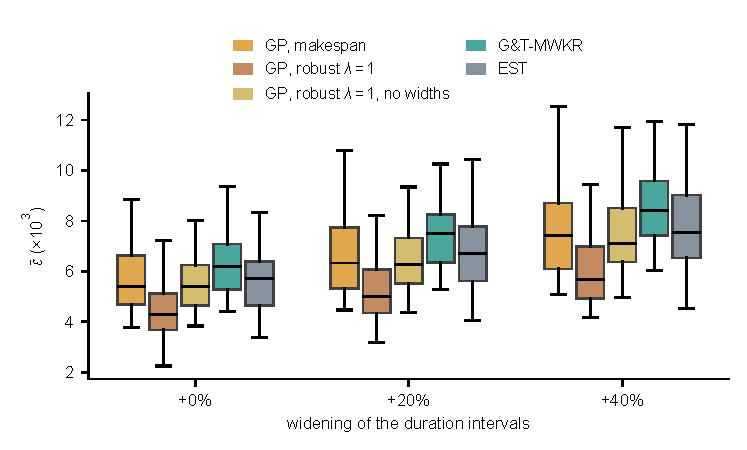
\includegraphics[width=\linewidth]{figures/fig_robustness_box.pdf}
\caption{Per-instance $\bar\varepsilon$ by method, with the duration
intervals at their nominal widths and widened by $+20\%$ and $+40\%$.
The robust $\lambda{=}1$ entries are the narrowest
rule of that arm and its counterpart evolved without the width
terminals, as in Table~\ref{M-tab:robustness}.}
\label{fig:robustness}
\end{figure}

Figure~\ref{fig:robustness} shows the per-instance $\bar\varepsilon$
distributions. The ordering is stable as uncertainty grows, and the
advantage of the robust rule widens with it: at $+40\%$ its deviation is
$6.08$ against $7.57$ for the makespan rule and $8.58$ for G\&T-MWKR.

\section{Asymmetric intervals}
\label{sec:asym}

Every instance used so far carries an interval symmetric about its
crisp value, so what the width terminals contribute could belong to the
generator rather than to the problem. The four arms of
Sections~\ref{M-sec:ablation} and~\ref{M-sec:frontier} were therefore
re-evolved on the asymmetric counterparts of TA11--TA14 described in
Section~\ref{M-sec:instances}, with the same configuration and fifteen
seeds per arm rather than thirty, a reduction imposed by the computational cost. Table~\ref{tab:asym} reports them over all 70 asymmetric
instances, with the executed deviation estimated from $400$ realizations
of the fixed processing order. Levels of $\RE$ do not compare across the
two benchmarks, since the right skew raises the expected makespan while
the crisp lower bound does not move and every arm sits some six points
higher; only the contrast between arms within a benchmark is meaningful.

\begin{table}[!htb]
\centering\small
\caption{The four arms re-evolved on asymmetric intervals and
evaluated over the 70 asymmetric instances: mean $\pm$ sd across 15
seeds of $\RE$, of the relative width of the predicted makespan
interval, and of the absolute deviation of the executed makespan.}
\label{tab:asym}
\begin{tabular}{lccc}
\toprule
Arm & RE (\%) & Width (\%) & $|\Delta|$ \\
\midrule
Makespan, full & $25.08 \pm 1.42$ & $13.23 \pm 0.72$ & $13.36 \pm 0.64$ \\
Makespan, no width & $23.90 \pm 1.18$ & $13.08 \pm 0.20$ &
$13.06 \pm 0.26$ \\
Robust $\lambda{=}1$, full & $25.93 \pm 1.18$ & $12.67 \pm 0.20$ &
$12.75 \pm 0.27$ \\
Robust $\lambda{=}1$, no width & $23.89 \pm 1.06$ & $12.97 \pm 0.18$ &
$13.03 \pm 0.16$ \\
\bottomrule
\end{tabular}
\end{table}

The main result is reproduced. Under the robust objective the
width terminals narrow the predicted interval from $12.97$ to $12.67$
($z=-3.59$, $|r|=0.77$) and the executed deviation from $13.03$ to
$12.75$ ($z=-2.80$, $|r|=0.60$), and the robust arm improves on the
makespan arm carrying the same terminals by $0.55$ points of width and
$0.61$ time units of deviation ($z=-3.59$, $|r|=0.77$ for the
latter). These five contrasts survive Holm's correction over the nine
Mann--Whitney tests of the table, the largest adjusted $p$ among them
being $0.0273$. The robustness that the width terminals make
attainable, and the objective under which they attain it, therefore do
not depend on the symmetric generation scheme.

Under the makespan objective the results are weaker than on the symmetric benchmark. There, the width terminals made the predicted
interval slightly but significantly narrower even though that objective
does not reward it (Section~\ref{M-sec:ablation}); here they do not
($13.23$ against $13.08$, $p=0.59$), nor do they reduce the executed
deviation ($13.36$ against $13.06$, $p=0.17$), and they cost $1.18$
points of $\RE$, a difference that does not survive the correction
($p=0.14$ adjusted). The negative result for expected makespan holds on
both benchmarks, and the remaining results are consistent with the boundary of
Section~\ref{M-sec:frontier}: where the objective does not price width,
the smaller terminal set is the better choice.

\section{Per-instance results}
\label{sec:perinstance}
Table~\ref{tab:perinstance} lists, for each of the 70 interval Taillard
instances, the crisp lower bound and the single-pass $\RE$ (\%) of the
evolved rule and of the two strongest baselines: EST, the best of the
plain dispatching rules, and G\&T-MWKR, the best baseline overall.

\begin{table}[!htb]
\centering\scriptsize
\caption{Per-instance $\RE$ (\%) of the evolved rule (GP) and of the two
strongest baselines, EST and G\&T-MWKR (single deterministic pass). LB is
the crisp Taillard lower bound.}
\label{tab:perinstance}
% 35 filas: a interlineado normal el float sobresale 19.8pt de la caja de
% texto y se come el numero de pagina
\renewcommand{\arraystretch}{0.92}
\setlength{\tabcolsep}{4pt}
\begin{tabular}{lrrrr@{\hskip 0.9em}|@{\hskip 0.9em}lrrrr}
\toprule
Inst. & LB & EST & G\&T & GP & Inst. & LB & EST & G\&T & GP \\
\midrule
TA1 & 1231 & 49.9 & 26.1 & 19.3 & TA36 & 1819 & 41.1 & 42.8 & 23.8 \\
TA2 & 1244 & 24.9 & 27.8 & 14.2 & TA37 & 1771 & 43.4 & 35.6 & 18.4 \\
TA3 & 1218 & 33.0 & 33.2 & 14.1 & TA38 & 1673 & 45.0 & 28.0 & 20.1 \\
TA4 & 1175 & 32.0 & 27.7 & 13.0 & TA39 & 1795 & 46.6 & 28.9 & 22.4 \\
TA5 & 1224 & 27.2 & 33.0 & 14.7 & TA40 & 1651 & 46.9 & 42.3 & 26.1 \\
TA6 & 1238 & 26.8 & 18.2 & 13.7 & TA41 & 1906 & 44.6 & 45.0 & 33.4 \\
TA7 & 1227 & 30.7 & 26.1 & 17.7 & TA42 & 1884 & 71.1 & 38.1 & 24.3 \\
TA8 & 1217 & 23.7 & 25.0 & 14.8 & TA43 & 1809 & 68.7 & 39.8 & 22.3 \\
TA9 & 1274 & 37.7 & 28.2 & 20.0 & TA44 & 1948 & 52.1 & 34.7 & 25.8 \\
TA10 & 1241 & 37.0 & 22.1 & 15.4 & TA45 & 1997 & 50.2 & 33.7 & 14.9 \\
TA11 & 1357 & 56.2 & 30.7 & 17.5 & TA46 & 1957 & 60.8 & 31.6 & 22.4 \\
TA12 & 1367 & 48.8 & 34.6 & 17.6 & TA47 & 1807 & 46.8 & 30.1 & 25.6 \\
TA13 & 1342 & 60.2 & 26.9 & 13.3 & TA48 & 1912 & 59.1 & 33.7 & 21.1 \\
TA14 & 1345 & 39.5 & 29.7 & 13.2 & TA49 & 1931 & 51.0 & 35.3 & 20.1 \\
TA15 & 1339 & 48.1 & 30.6 & 16.7 & TA50 & 1833 & 61.4 & 46.2 & 31.3 \\
TA16 & 1360 & 45.2 & 34.0 & 15.6 & TA51 & 2760 & 33.8 & 34.7 & 23.2 \\
TA17 & 1462 & 58.9 & 17.7 & 13.9 & TA52 & 2756 & 38.0 & 26.5 & 12.7 \\
TA18 & 1377 & 43.8 & 31.8 & 23.6 & TA53 & 2717 & 34.1 & 18.3 & 11.8 \\
TA19 & 1332 & 45.8 & 29.3 & 20.0 & TA54 & 2839 & 20.9 & 16.1 & 8.2 \\
TA20 & 1348 & 45.7 & 24.1 & 15.1 & TA55 & 2679 & 31.7 & 29.2 & 15.5 \\
TA21 & 1642 & 33.4 & 28.0 & 20.2 & TA56 & 2781 & 34.8 & 19.8 & 10.9 \\
TA22 & 1561 & 44.2 & 30.8 & 17.4 & TA57 & 2943 & 32.9 & 20.0 & 9.6 \\
TA23 & 1518 & 42.8 & 35.3 & 17.8 & TA58 & 2885 & 37.4 & 26.3 & 13.6 \\
TA24 & 1644 & 56.3 & 23.8 & 14.1 & TA59 & 2655 & 26.6 & 28.2 & 16.7 \\
TA25 & 1558 & 45.8 & 33.8 & 16.6 & TA60 & 2723 & 41.7 & 19.8 & 15.5 \\
TA26 & 1591 & 42.8 & 31.2 & 26.9 & TA61 & 2868 & 45.7 & 25.4 & 15.4 \\
TA27 & 1652 & 50.0 & 31.1 & 21.4 & TA62 & 2869 & 43.0 & 27.6 & 17.2 \\
TA28 & 1603 & 36.8 & 26.8 & 12.4 & TA63 & 2755 & 38.8 & 23.8 & 13.4 \\
TA29 & 1583 & 28.8 & 32.0 & 17.2 & TA64 & 2702 & 38.2 & 28.4 & 12.2 \\
TA30 & 1528 & 34.2 & 36.1 & 17.0 & TA65 & 2725 & 42.9 & 30.0 & 20.5 \\
TA31 & 1764 & 30.7 & 34.4 & 24.5 & TA66 & 2845 & 41.8 & 28.0 & 11.9 \\
TA32 & 1774 & 42.7 & 33.3 & 19.0 & TA67 & 2825 & 31.7 & 26.1 & 15.2 \\
TA33 & 1788 & 51.3 & 34.8 & 27.5 & TA68 & 2784 & 50.1 & 19.1 & 10.6 \\
TA34 & 1828 & 45.9 & 31.8 & 20.7 & TA69 & 3071 & 35.3 & 22.8 & 12.9 \\
TA35 & 2007 & 30.3 & 24.1 & 8.4 & TA70 & 2995 & 42.9 & 23.4 & 16.7 \\
\bottomrule
\end{tabular}
\end{table}

\section{The seeded genetic algorithm over time}
\label{sec:semilla}

Table~\ref{tab:semilla} compares the genetic algorithm seeded with the
rule's permutation against the unseeded one at several budgets on the
four instance sets of Section~\ref{M-sec:budget} of the article. The
seed gives a significant advantage on every set after one second per
instance, for longer the larger the instance, and none from $100$~s per
instance on. The tests at different budgets are not corrected for
multiplicity; with 10 instances the smallest attainable two-sided $p$ is
$0.002$, the value repeated in the first rows.

\begin{table}[!htb]
\centering\small
\caption{The seeded genetic algorithm against the unseeded one: number
of instances on which the seeded version is better and, in parentheses,
the two-sided paired Wilcoxon $p$, with the instance as unit (the mean
over its runs). A dash marks a budget beyond the horizon of the set.}
\label{tab:semilla}
\begin{tabular}{lcccc}
\toprule
Seconds & Classical (12) & $15{\times}15$ (10) & $30{\times}15$ (10) & $50{\times}15$ (10) \\
\midrule
1 & 11 (0.001) & 10 (0.002) & 10 (0.002) & 10 (0.002) \\
3 & 8 (0.064) & 10 (0.002) & 10 (0.002) & 10 (0.002) \\
10 & 5 (0.970) & 6 (0.625) & 9 (0.004) & 10 (0.002) \\
30 & 5 (0.970) & 6 (0.625) & 5 (0.846) & 9 (0.006) \\
100 & 6 (0.791) & 5 (1.000) & 4 (0.432) & 8 (0.064) \\
300 & 6 (0.791) & 5 (0.846) & 5 (0.846) & 6 (0.432) \\
1000 & --- & --- & 4 (0.846) & 6 (0.625) \\
End of horizon & 6 (0.791) & 3 (0.625) & 4 (0.375) & 7 (0.432) \\
\bottomrule
\end{tabular}
\end{table}

\section{Ablation results}
\label{sec:ablationtab}

Table~\ref{tab:ablation} gives the means of the arms compared seed by
seed in Figure~\ref{M-fig:ablation} of the article.

\begin{table}[!htb]
\centering\small
\caption{Ablations of the interval machinery (30 independent evolutions
per arm; Mann--Whitney tests between arms): the terminal ablation under
two fitness objectives, and the crisp-midpoint control, evolved with
scalar fitness and no interval information, tested against the
interval-trained arm above it. \emph{Width} is the relative width of
the predicted makespan interval.}
\label{tab:ablation}
% la celda del test de RE bajo el objetivo robusto ensancha la tabla 12.9pt
% sobre los 360pt de caja; a 4pt mide 356.9pt
\setlength{\tabcolsep}{4pt}
\begin{tabular}{llcc}
\toprule
Fitness objective & Terminal set & RE (\%) & Width (\%) \\
\midrule
\multirow{3}{*}{Makespan $E[\mathbf{C}_{\max}]$}
 & full & $18.99 \pm 1.33$ & $12.41 \pm 0.30$ \\
 & without widths & $18.66 \pm 1.08$ & $12.62 \pm 0.23$ \\
 & \textit{test} & \textit{n.s.} ($z=0.67$) & $z=-2.96$, $p<0.01$ \\
\midrule
\multirow{2}{*}{Midpoint control}
 & without widths & $18.63 \pm 0.99$ & $12.55 \pm 0.17$ \\
 & \textit{test} & \textit{n.s.} ($z=-0.12$) & \textit{n.s.} ($z=-1.26$) \\
\midrule
\multirow{3}{*}{Robust, Eq.~\eqref{M-eq:robustfit}}
 & full & $19.62 \pm 1.52$ & $12.04 \pm 0.75$ \\
 & without widths & $18.42 \pm 0.87$ & $12.47 \pm 0.20$ \\
 & \textit{test} & $z=3.59$, $p<0.001$ & $z=-2.99$, $p<0.01$ \\
\bottomrule
\end{tabular}
\end{table}

\end{document}
